\documentclass[12pt]{article}
\usepackage[
backend=biber,
style=alphabetic,
]{biblatex}
\addbibresource{sample.bib} %Imports bibliography file
% fonts

\usepackage[scaled=0.92]{helvet}   % set Helvetica as the sans-serif font
\renewcommand{\rmdefault}{ptm}     % set Times as the default text font

\usepackage[T1]{fontenc}
\usepackage{amsmath}
\usepackage{amsfonts}

% page numbers
\usepackage{fancyhdr}
\fancypagestyle{newstyle}{
\fancyhf{} % clear all header and footer fields
\fancyfoot[R]{\vspace{0.1in} \small \thepage}
\renewcommand{\headrulewidth}{0pt}
\renewcommand{\footrulewidth}{0pt}}
\pagestyle{newstyle}

% geometry of the page
\usepackage[top=1in,
            bottom=1in,
            left=1in,
            right=1in]{geometry}

% paragraph spacing
\setlength{\parindent}{0pt}
\setlength{\parskip}{2ex plus 0.4ex minus 0.2ex}

% useful packages
\usepackage{natbib}
\usepackage{epsfig}
\usepackage{url}
\usepackage{bm}

\renewcommand{\floatpagefraction}{.8}%

\begin{document}

\large \textbf{Synthetic Control Methods for Estimating the Effect of the Change of Leadership in Early-stage Startups} \\
Chenyang Zhu (cz2641) \\
\today

\vspace{0.1in}

\normalsize


\begin{abstract}
    A new leadership is usually considered as an important signal of changes in an early stage startup, but whether such treatment can cause a substantial growth of the company remains a speculation rather than science. In this paper, we use the financing history of 1,514 early-stage startups from 2003-2013 in the US. We use synthetic control method with matrix completion \cite{athey2021matrix} to estimate the average treatment effect of the treated (ATT) on the effect of changing leaderships. We also utilize the BERT \cite{devlin2018bert} embedding of startup's websites as text confouding to adjust for the estimate. In contrary to most industry's belief, changing leadership in early-stage startup has no causal effect superior growth of the startup, and in some cases worse performance.

\textbf{Keyword}: Synthetic Control, Natural Language Processing, Causal Inference.
\end{abstract}



% 1. Background. Why is this an important question?
% 2. Has anyone researched this problem before?
% 3. What are some of the problems they cannot solve?
% 4. Can our research solve this problem? Yes.

\section{Introduction}
One of the biggest counterfactual question people frequently ask about in business is "What if we change the leadership team?" Yet, a simple question like this remained unanswerable by decades of wise leaders and well-trained analysts in the industry. Seeking a framework to answer counterfactual questions in business is the main goal of this project.

In particular, this project focuses on estimating the causal effect of changing a new CEO on the financing growth of the startup. This project uses a matrix completion version of synthetic control methods \cite{athey2021matrix} with data from the financing history of 1,514 early stage startups from a free startup database Crunchbase. The first 5 rounds of financing (i.e. Series A, B, C) of these startups are studied, and 44 startups changed their leadership during the observed period in only one of the rounds. Therefore we consider the problem to be a staggered adoption problem within the synthetic control field. The websites of these startups are also collected to serve as an extra source of confounders, where a BERT model is used to generate embeddings \cite{devlin2018bert} that are considered as the inputs to the synthetic control method.

We tested three model variants within the synthetic control methods, and none of the models find significant causal effects of changing leadership in early stage startups, in contrary to the common belief of the industry. In some cases, changing leadership too early or too late tend to lead to disastrous effect on the growth of the startup.

Such estimation problem might be more common in other research domains, but it is historically challenging for business data for several reasons. First, most data in the business world are unstructured texts from news and websites. There were no good methods for dealing with these types of data except for manual feature engineering. Second, feature engineering might not always be helpful because many variables were and remains to be un-collectable and uncontrollable. This is because of the lack of open information required by regulators around the world and the tendency of keeping corporate operation secret. Third, and even worse, the uncontrollability cannot be solved by doing any controlled experiments because real-world business cannot be intervened upon. These inherently challenging problems has historically expelled business research from serious science, even though the questions in this field affects everyone's socio-economic life.

Only in recent years, with the advance of natural language models and causal inference, some researchers start to analyze these counterfactual answers with more scientific approaches. In a broader picture, researchers categorize business causal questions into two domains \cite{gelman2013ask}. On one hand, the reverse causal problems, such as "What caused the sales to drop?", seeks to find the cause of a phenomenon. On the other hand, the forward causal problem wants to know the effect of a policy, such as "What if we use recyclable boxes in our delivery?" Both directions are important in a business and are less explored because causal inference is different from traditional parameter estimates in many social science and business questions \cite{athey2015machine}.

This project focuses on the forward causal problem in the pursuit of an understanding of how company's strategy could change its path of growth in the future. Prior to this project, \cite{guzman2021treatment} is one of the first researchers in this area. They use the TF-iDF metrics to measure the distance between the website of startups, and estimate the causal effect of founding strategies and the change of strategies on these startups. We follow similar research procedures. This project aims to provide a practical applied causality solution to a set of practical counterfactual problems, and leaves theoretical advancement to future research.

To this end, the paper is structured in several sections. In Section \ref{sec:methods}, we describe the research methodology, including synthetic control with matrix completion, adding covariates to the optimization problem, and using text as confounding. In Section \ref{sec:estimate}, we present the data collection and preprocessing procedures. We introduce the specifications of the three models we consider in this project. We then present the estimation the treatment effect of changing leadership in early-stage startups. In Section \ref{sec:placebo}, we show the placebo test for the synthetic control method, and discuss the limitation of the model. In Section \ref{sec:discuss}, we discuss further research directions and business implications.


\section{Research methods}
\label{sec:methods}

\subsection{Synthetic control without confounders}
Synthetic Control is particularly suitable for answering this question. First, The investigation of leadership in corporations should be answered in time series, simply because any policy deployed by the leadership usually requires a period of time to show effects. This aspect differentiates our research problem from problems that could be answered by a two-phase difference in difference model. Second, it is impossible to conduct controlled experiments on the change of leadership in the real world. Researchers have to rely on panel data on non-randomized real world data. The lack of experiments refrains our investigation from using more traditional methods. The above two points lead us to use synthetic control methods.

In this project, we use the matrix completion method for causal panel data (\cite{athey2021matrix}), which is slightly different from the usual compare and predict pipeline. This method considers a matrix $Y$ of dimension $N \times T$, where $N$ is the number of samples, and $T$ is the number of timestamps. The idea is to combine the traditional synthetic control methods, including the horizontal regression and the vertical regression, into a factor model with matrix completion techniques. The fixed effect model has parameter $\Gamma = [\gamma_1, \dots, \gamma_T] \in \mathbb{R}^T$ for each timestamp, $\Delta =[\delta_1, \dots, \delta_N] \in \mathbb{R}^{N}$ for each sample, and an error term $\epsilon_{it}$. In other words,
\begin{align*}
    Y_{it} = \gamma_i + \delta_t + \epsilon_{it}
\end{align*}
Thus, the idea is to find such matrix $L^*$ that satisfies $Y = L^* + \varepsilon$, where $\mathbb{E}[\varepsilon | L^*]=0$. The matrix completion method then boils down to the following optimization problem.
\begin{align}
    \label{eq:noCov}
    (L^* , \Gamma^*, \Delta^*) = \arg\min_{L, \Gamma,\Delta} \bigg[ \frac{1}{|\mathcal{O}|} \|P_\mathcal{O}(Y-L-\Gamma 1_T^\bot -1_N\Delta^\top)\|_F^2+\lambda \|L\|_* \bigg]
\end{align}
where the $\|\cdot\|_*$ represents nuclear norm, and $\|\cdot\|_F$ represents the Fr\"{o}benius Norm.
There are two things to notice before we use this method. First, the method itself does not render any causal interpretation. The matrix completion only intends to find the potential outcome for the counterfactual world, and researchers need to re-interpret the result in the Causal framework. Second, the R package offered by the authors, \texttt{MCPanel} completes the matrix without taking any confounders into consideration. We will use this method as a baseline, and add confounders in the next model.

\subsection{Synthetic control with covariates}
\label{scc}
We then modify the code of the matrix completion algorithm to add the covariates \cite{athey2021matrix}. In addition to the previous setup, we also observe a covariate matrix $X \in \mathbb{R}^{N \times P}$, where $N$ is the number of startups, and $P$ is the number of covariates. The model we consider is a matrix completion problem with covariates,
\begin{align*}
    Y_{it} = L_{it}^* + \sum_{p=1}^P X_{ip}h_p^* + \gamma_i^* + \delta_t^* + \varepsilon_{it} \text{,   } \forall i \in N, t\in T
\end{align*}
To rewrite in a matrix form is, let $L^* \in \mathbb{R}^{N \times T}$, $\Gamma^* \in \mathbb{R}^{N \times 1}$, $h^* \in \mathbb{R}^{P \times 1}$, and $\Delta^* \in \mathbb{R}^{T\times 1}$.
\begin{align*}
    Y = L^* + Xh^* + \Gamma^* 1_T^\top  + 1_N(\Delta^*)^\top + \varepsilon
\end{align*}
Our goal is to estimate the matrix $L^*$, $h^*$, $\Delta^*$, $\Gamma^*$, \cite{athey2021matrix}
\begin{align}
    \label{fuc:min}
    \min_{h, L, \Delta, \Gamma} \bigg[ \sum_{(i, t)\in \mathcal{O}} \frac{1}{|\mathcal{O}|}(Y_{it} - L_{it}^* - \sum_{p=1}^P X_{ip}h_p^* - \gamma_i^* - \delta_t^*)^2  + \lambda_L \|L\|_* + \lambda_h \|h\|_{1,e} \bigg]
\end{align}
Equation (\ref{fuc:min}) simply adds a covariate matrix to Equation (\ref{eq:noCov}). While the authors did not include examples in the paper, we observe a better fit of the data when taking the covariates into consideration and we show more details in Section \ref{sec:placebo}.

\subsection{Text as confounding}
We also consider text as confounding in this work. While the causal representation learning field is burgeoning with new papers every other week, we realized that most of these algorithms requires sufficiently large computation power. In addition, to connect with existing synthetic control methods, perhaps using text as confounding is a good way to start. This is especially useful in domains that historically lack structured information, such as the startup industry, where all data about a startup is hidden inside news, company websites, or social media.

In the field of text as confounding, some researchers suggest that texts can be used to adjust for confounding through propensity scores \cite{weld2020adjusting}. Others suggest a plug-and-play solution that uses embeddings or topic models as confounders \cite{keith2020text,veitch2020adapting}. In this project, for lack of computational power, we will use the out-of-box BERT model \cite{devlin2018bert} as confounding, and leave the computationally intensive approach for future explorations. After getting the embedding $E \in R^{N \times H}$, where $H = 768$ for BERT models, we concatenate the embedding $E$ with the covariate matrix $X$ and feed it into the model specified in Equation (\ref{fuc:min}).

\section{Estimating the effects of change of leadership}
\label{sec:estimate}

\subsection{Data collection}

To estimate the effect of the change of leadership in early-stage startups, we used a free data set online that collected more than 190,000 startups in the US from 2003 to 2013 from the public website Crunchbase. We filtered startups that have received at least one funding rounds and remained in operation up until December 2013. This allows us to assume continuous operation during the period of our data set and exclude possible exogenous interference such as acquisition or bankruptcy.

For each of these startups, we obtain a time series of their founding rounds (i.e. Series A, B, C) that contains total money funded and corresponding investors. These time series are discrete, with gaps between each round as close as one month or as large as several years. To process the timeline of different startups in batches, we adopted a numerical sequencing of series to represent rounds of funding instead of raw timestamps, so that the funding timelines for different startups are aligned. 99\% of the startups only have 5 rounds of funding, so we restrict our attention to the first five rounds.

\begin{figure}
    \centering
    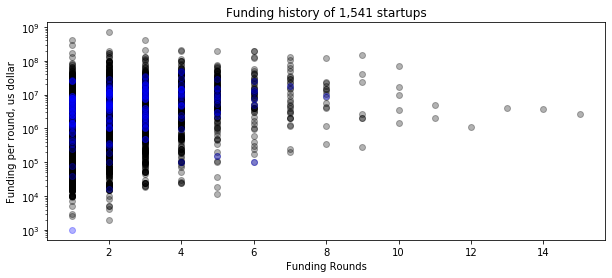
\includegraphics[width=\textwidth]{figures/history.png}
    \caption{Funding history of the data set. The x-axis is the founding rounds. The y-axis is the funding per round after log transformation. Black dots represent the control group, and blue dots represent the treatment group. }
    \label{fig:history}
\end{figure}

Our goal is to study how leadership changes would cause early-stage startups. The treatment is the recorded change of the CEO. We obtain the CEO data from the same data set. We then convert the inauguration time of the new leadership into the same numerical sequencing as the startups. Of the total  1,541 startups, we observe that 1,497 startups did not change any CEO, and the rest 44 startups changed leadership. For the purpose of this project, we assume that the treatment is binary. In other words, it is assumed that there is no inherently good CEO or bad CEO. In practice, most new CEO's are considered the hero or the heroine of the company (before they are proven to be as worse as the previous one). It is practically hard to label a CEO into a scale of goodness.

Notice that different startups now receive their treatment in different rounds, so our problem can be defined as Staggered Adoption problem \cite{athey2022design}, which estimates the treatment effect of the same treatment but having occurred at different timestamps. This is not a typical setup of the synthetic control method, but it would be interesting to explore with the new proposed matrix completion algorithm.

Figure \ref{fig:history} shows the funding history of each startup. We choose the response variable to be the percent change of funding in phase $t$ compared with phase $t-1$. The rationale is that the funding a startup gets in a particular round is proportional to the valuation of the startup. If funding goes up, it usually means that the valuation of the startup goes up, which is an indicator of good leadership. We use a percentage change of this valuation, to measure the value created under this leadership in the considered period. This construction gives us a time series matrix of $N=1,541 \times T=4$ which we will call $Y$.

Figure \ref{fig:analytics} shows the average change of funding led by changing leadership before each phase. The funding trend is downward slopping, because we are measuring the growth rate of the valuation, and the growth rate for a company tends to decrease in the long run. The treatment group underperforms the control group in all except the last scenario, and there is little material difference between the control and treatment groups. Before the change of leadership, both two groups have similar valuation trajectories, and there is not much differentiation after the change of leadership.

We also downloaded the company's website page as an extra source of confounding. The reason for using text data is that startup data usually are not well-documented and well structured, as compared with public companies. This has historically contributed to the difficulty of analyzing the startup ecosystem. This approach of using website data is similar to the approach of \cite{guzman2021treatment}. We first use Clearbit services to find the domain of the company in our dataset. Since startups usually change their business scope frequently, we use Wayback services to find the website HTML when the company was first founded. These website HTML files are transformed into pure texts which are later used as input to the BERT model for the embedding.


\begin{figure}
    \centering
    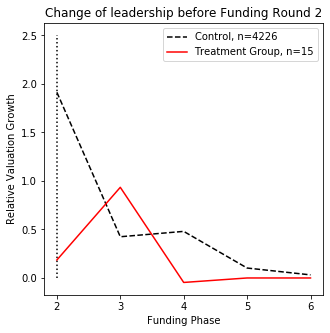
\includegraphics[width=.45\textwidth]{figures/r2.png}
    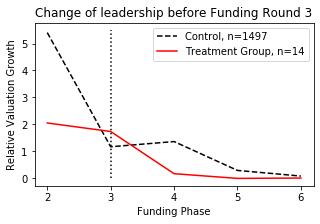
\includegraphics[width=.45\textwidth]{figures/r3.png}
    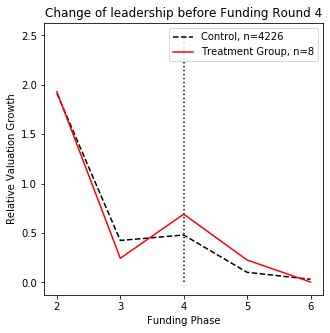
\includegraphics[width=.45\textwidth]{figures/r4.png}
    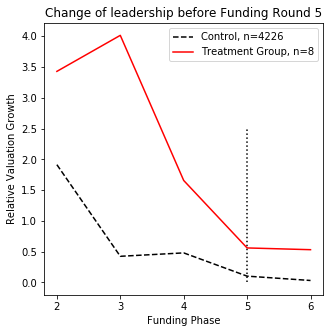
\includegraphics[width=.45\textwidth]{figures/r5.png}
    \caption{The average change of funding after changing leadership in each round. The y-axis is the relative growth of the company. The x-axis is the funding round. The red solid line is the treatment group, and the dotted black line is the control group. The vertical dotted lines indicate the time of the treatment. }
    \label{fig:analytics}
\end{figure}

\subsection{Model specification}
We consider three models in this project.

\textbf{Model 1}. The first model is the vanilla synthetic control algorithm from \cite{athey2021matrix}. We use the \texttt{MCPanel} package from the authors. The input of this algorithm is the time series we collected with $N$ samples and $T$ timestamps, $Y \in \mathbb{R}^{N \times T}$. We create a treatment matrix $\mathbf{T} \in \{0, 1\}^{N \times T}$ of binary variables, where the samples in the treatment group are set to 1 at the round they were treated. Since all startups were only treated once, $\sum_{i\in N, t\in T} \mathbf{T}_{it} = N$. We train the algorithm considering fixed effects for each startup. We use the \texttt{mcnnmcv} for cross validation with 40 choices of $\lambda_L$, the covariate for the penalty term $\|L\|_*$.

\textbf{Model 2}. In the second model, we add the only covariate in the data set, the category of the startup. The covariates are stored as one-hot vectors in $X \in \mathbb{R}^{N \times P}$. In our case, we have $P = 42$ one hot vectors indicating the category of startups. The model is presented in Equation \ref{fuc:min} in Section \ref{scc}. We use PyTorch to write the code and train the model. We first  randomly initiate the parameters and use stochastic gradient descent with learning rate 0.01 to minimize the objective function. We notice relatively poor convergence in the model.

\textbf{Model 3}. In the third model, we consider a standard uncased BERT model as embeddings. We take the text data from the startup's website, truncate the website to 512 characters, and feed it into BERT model. For each website, we take the embedding of the first token \texttt{[CLS]} of size 768. We then concatenate the embedding with the categorical one-hot labels to get the covariate matrix $X \in \mathbb{R}^{N \times P}$, where $P = 768 + 42 = 810$. Then we fit the synthetic control model the same way as Model 2.

In a nutshell, Model 1 is the vanilla synthetic control method with matrix completion. Model 2 adds the category of the startup using one-hot vectors. Model 3 adds startup's website as confounders.

After obtaining the estimation $L^*=\hat Y^0$, we then compute the average treatment effect on treated (ATT) for round $t$,
\begin{align}
\label{eq:att}
\text{ATT}_t = \mathbb{E}[Y^{1}_t - \hat  Y^0_t | \mathbf{T}_t = 1]
\end{align}
for sample in the treatment group, where $Y^1_t$ is the treated response variable from real world for round $t$ and $\hat Y^0_t$ is the estimation from the algorithm.


\subsection{Experiment results}

\begin{figure}
    \centering
    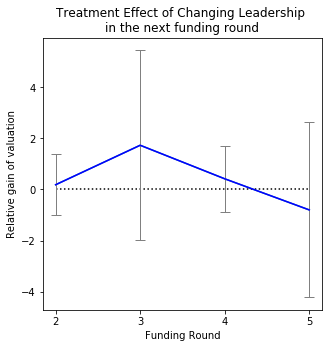
\includegraphics[width=.3\textwidth]{figures/L01.png}
    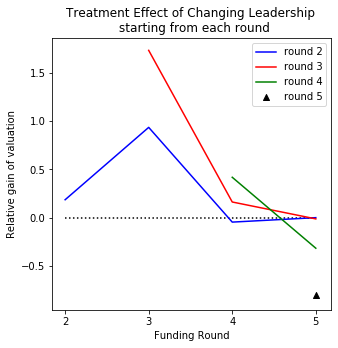
\includegraphics[width=.31\textwidth]{figures/L03.png}
    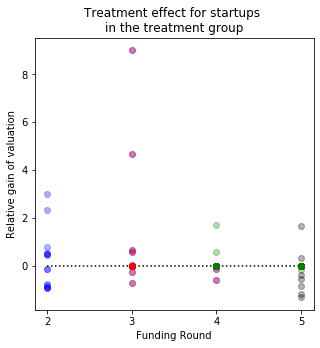
\includegraphics[width=.32\textwidth]{figures/L04.png}
        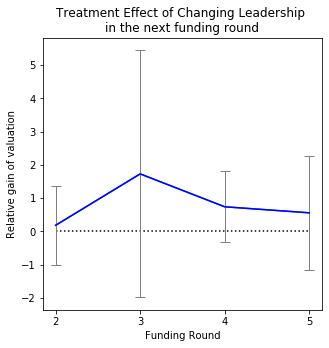
\includegraphics[width=.3\textwidth]{figures/L11.png}
    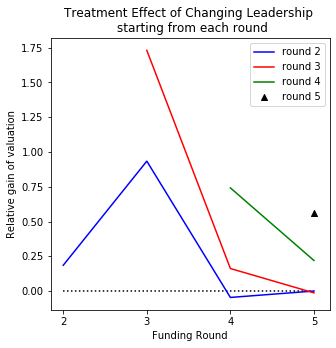
\includegraphics[width=.31\textwidth]{figures/L13.png}
    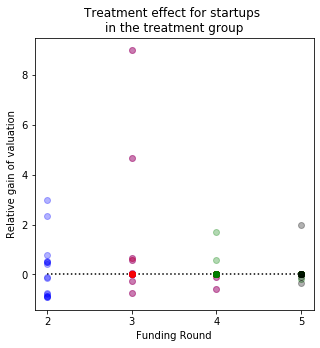
\includegraphics[width=.32\textwidth]{figures/L14.png}
    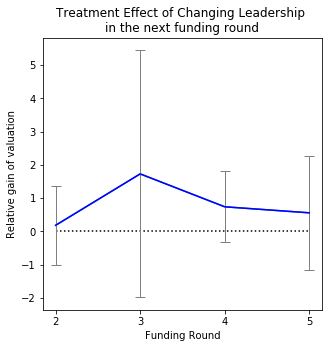
\includegraphics[width=.3\textwidth]{figures/L21.png}
    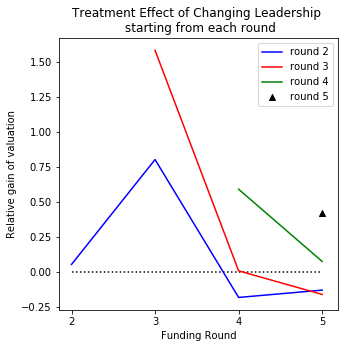
\includegraphics[width=.31\textwidth]{figures/L23.png}
    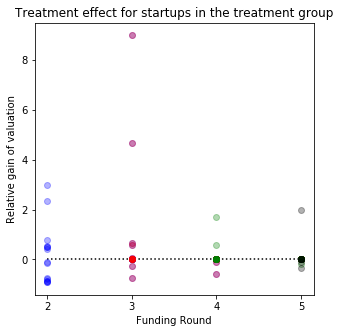
\includegraphics[width=.32\textwidth]{figures/L24.png}
    \caption{Treatment effect of changing leadership before each funding round. From top to bottom represents the estimation result for model 1, 2 and 3. From left to right,  a) The average treatment effect for the treated, defined in Equation (\ref{eq:att}). b) The average treatment effect for the treated from the treated round to the last round. c) The scatter plot of the average treatment effect estimation.}
    \label{fig:trNoCon}
\end{figure}

The results are shown in Figure \ref{fig:trNoCon}. The three figures in Column (a) show that there is no significant treatment effect of the change of leadership to the growth of the startup in any of the models. The three figures in Column (b) show that there is even a slightly negative effect after changing leadership in the long run. Column (c) gives us the full picture of the estimation. Almost all treatment effects are either negative or close to 0.

In terms of the performance of models, we observe that the three models actually have very similar results. Model 2 and Model 3, in particular, have very similar results. It shows that the the matrix completion method with simple covariates could capture enough information without using the text data.

The business implication of our result is straight-forward. Startups generally don't benefit from changing a CEO. Some startups would even have worse performance had they changed their CEOs. If the startup has to change the CEO for whatever reason, it would be wise to do it during the growth stage of the startup and avoid doing it too soon or too late.


\section{The placebo test}
\label{sec:placebo}
The Placebo Test, as proposed in various synthetic control papers \cite{abadie2010synthetic,abadie2003economic} is designed to test the significance and validity to use the synthetic control method. The method applies the synthetic control estimation to the control group to regenerate an estimation for each sample in the control group. If the gap between the generated sample and the true sample is large, that means synthetic control methods are unable to regenerate the feature of the controlled sample and researchers should not use synthetic control methods for the problem.

In our project particularly, we sample 100 startups from the control group. For each selected startup, we conduct the synthetic control prediction on these groups as if their leadership has been changed. We call their true trajectory of funding growth in the data set as "authentic" growth $Y$, and the predicted growth as "synthetic" $L^*$. We then calculate the $l_2$-norm of $\|Y - L^* \|_2$ as a way to measure the distance between $Y$ and $L^*$, as a way to measure the fit of the models. We repeat the above experiment 10 times for each model. Ideally, the authentic growth and the synthetic growth should be very similar $Y \approx L^*$, indicating that the synthetic control algorithm makes sense.

The result for model comparison is shown in Table \ref{tab:performance}. It shows that the synthetic model with categorical labels performs the best, in terms of recovering the sample from other samples in the control group. The reason that the text embedding model does not perform well could be that the embedding model is not trained for this particular task, and it could be that the website data added noise to the synthetic control method.

\begin{table}[]
    \centering
    \begin{tabular}{|c|c|c|c|} \hline
         & \textbf{Model 1} &\textbf{ Model 2 }& \textbf{Model 3}  \\ \hline
         & Synthetic Control  & Synthetic Control  & Synthetic Control \\
         & with no covariates &  with categorical labels & with text embeddings  \\ \hline
         $l_2$-norm $\|L - \hat L\|_2$ & 305.69 ($\pm$ 170.37) & 243.75 ($\pm$ 101.23) & 492.14 ($\pm$ 214.56) \\ \hline
    \end{tabular}
    \caption{Model Performance in the placebo test. Smaller $l_2$-norm indicates better fit on the data. The value in the parenthesis is the standard deviation of the $l_2$-norm. }
    \label{tab:performance}
\end{table}


\section{Discussion}
\label{sec:discuss}
The placebo test show that the synthetic control method in \cite{athey2021matrix} did not perform well in our data set. There are multiple reasons to this. First, the startup data is inherently heterogeneous, with different industries and directions. Thus, it is difficult to apply the matrix completion matrix to identify similar comparative cases, even with the help of embeddings. Second, the way we treated the startup data, in discrete time series, might also contribute to the high variability. Even if we restrict our scope to the first five series, some startups might secretly cease operation while others might not operate so well. These information is not included in our data set, and some may never be written down or documented at all.

Apart from the inherent difficulty of the problem and the fact that synthetic control might be the only way for us to understand the problem, it remains further research and application whether the method from \cite{athey2021matrix} works well with covariate matrix. On the other hand, the text embedding methods could also be further improved to models that are better trained on website and business data set. Other methods such as topic models should also be tested with the matrix-completion framework.

We consider this project as a new approach in broader business applications. The industry is historically haunted by poorly-structured text data, long-hour manual work, and careless conclusions. From the industry background of the author, counterfactual questions like "What if our startup changes the strategy?", "what if we change our leadership after several rounds of financing? Will investors still trust us?", and "what if we hire more people?" are encountered on an every-day basis. These questions are traditionally answered with "It depends", and followed by a practical step to look at "comparable companies", usually their websites. The idea is that if a similar company had the same problem and succeeded by taking step A, then step A probably will work for our clients too. It is horrible that nowadays these advice are given to companies without scientific approach, considering that most decisions are a bankrupt or IPO choice for early stage companies.

With synthetic control and natural language techniques, the author's hope is that these manual work of "matching" and "learning" could be automated. Although in this paper, the method seems to render very poor results, it is one step closer to the desired automation. The difficulty lies in the following key steps to iterate. How to select the correct comparable cases under the matrix completion framework? This seems to be a missing piece from \cite{athey2021matrix}, and more specifically how can text be of help? What can we learn from the burgeoning representation learning papers? These answers could only be understood by further research.

\section{Conclusion}
In this paper, we use synthetic control and natural language processing methods to find the treatment effect of the change of leadership in early-stage startups. We used a data set from Crunchbase that contains 1541 startups, and 44 of which have changed their CEO's during the first five rounds of financing events. In contrary to most industry practitioner's experience, We found no causal effect on the company growth after the inauguration of these new CEO's. We tested our hypothesis with three models, and found that using BERT embedding generated by startup's website failed to provide better estimation of the treatment effect. Further research include testing using better nlp techniques and experimenting with different synthetic control methods.

\medskip

% \bibliography{sample}
\printbibliography

\end{document}

%%% Local Variables:
%%% mode: latex
%%% TeX-master: t
%%% End:
